\begin{frame}
    \frametitle{Differenzverstärker}
    \framesubtitle{}
%    \begin{block}{Ziel:}
%        Verstärkung sehr kleiner Potentialunterschiede $\Delta V \approx 10\mu
%        V$ \\ $\rightarrow$ Differenzverstärker
%    \end{block}
%    \pause
%    \begin{figure}[H]
%    \begin{center}
%            \includegraphics[scale=0.2]{./img/schaltung/difver_1.png}
%    \end{center}
%    \end{figure}
%\end{frame}
%\begin{frame}
%    \frametitle{Differenzverstärker}
%    \framesubtitle{}
%    
    \begin{block}{Differenzverstärker}
        \begin{itemize}
            \item ähnelt dem invertiertem Verstärker
            \item bestimmt Potentialdifferenzen an den Anschlüssen
        \end{itemize}
    \end{block}
\end{frame}
\begin{frame}
\frametitle{Versuchsaufbau}
\framesubtitle{}
    \begin{block}{Versuch}
        \begin{itemize}
            \item Aufbau wurde mit DAQ-Box Verbunden
            \item Bestimmung von Gegentaktverstärkung, Gleichtaktverstäkrung
            und Gleichtaktunterdrückung
        \end{itemize}    
    \end{block}
    \begin{figure}[H]
    \begin{center}
            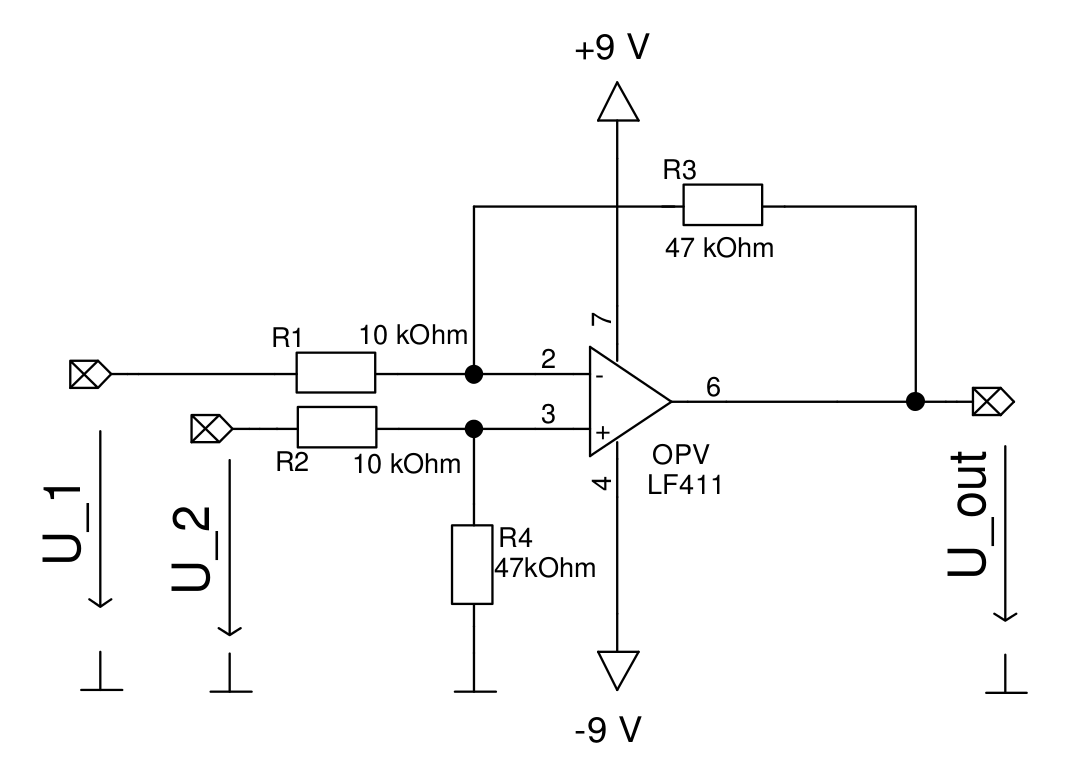
\includegraphics[scale=0.2]{./img/schaltung/dif_verst_1.png}
    \end{center}
    \end{figure}
\end{frame}
\begin{frame}
\frametitle{CMRR}
\framesubtitle{}
    \begin{columns}[c]
    \column{0.6\textwidth}
    \begin{block}{Gleichtaktunterdrückung}
         \begin{itemize}
             \item Gegentaktverstärkung:
             \begin{equation*}
                 G_{diff} = \frac{\partial U_{out}}{\partial U_{diff} } = -
                 \frac{R_3}{R_1}= -4.7
             \end{equation*}
             \item Gleichtaktverstärkung
             \begin{equation*}
                 G_{CM} =
             \end{equation*}
             \item Gleichtaktunterdrückung
             \begin{equation*}
                 CMRR= \frac{G_{|diff}|}{|G_{CM}|}=
             \end{equation*}
         \end{itemize}
    \end{block}
    \column{0.5\textwidth}
    \begin{figure}[H]
    \begin{center}
            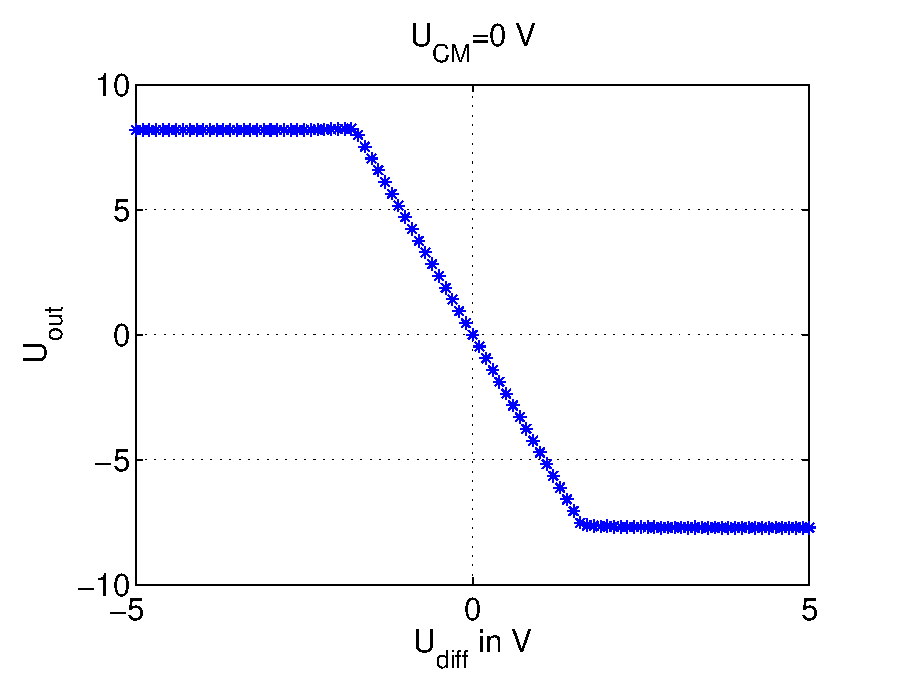
\includegraphics[scale=0.3]{./img/plots/Auf_3_Ucm_0.eps}
    \end{center}
    \end{figure}
    \begin{figure}[H]
    \begin{center}
            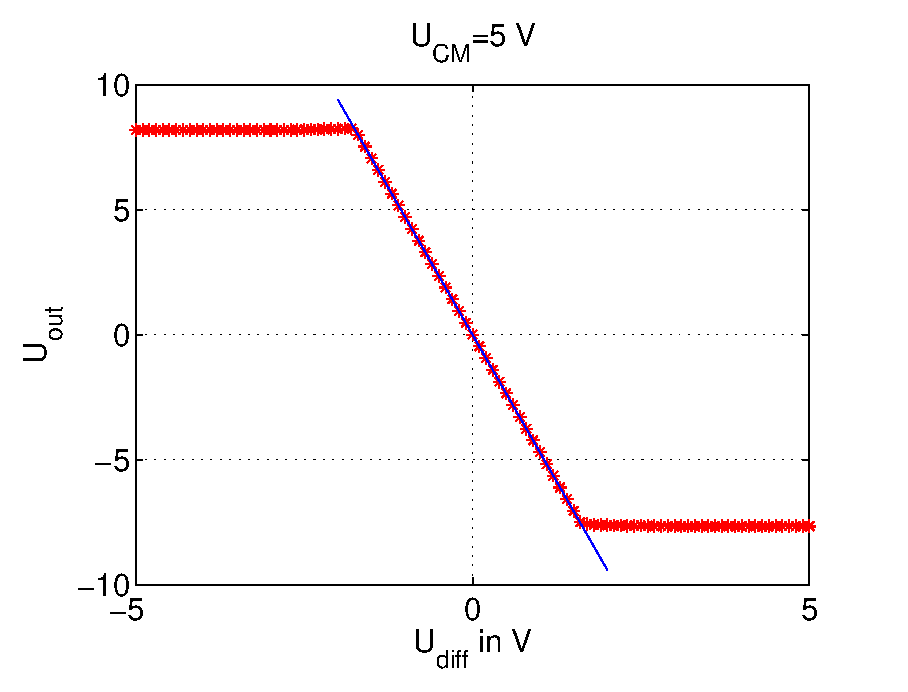
\includegraphics[scale=0.3]{./img/plots/Auf_3_Ucm_5.eps}
    \end{center}
    \end{figure}
    
    \end{columns}
\end{frame}
\begin{frame}
\frametitle{CMRR}
\framesubtitle{}
    \begin{columns}[c]
    \column{0.5\textwidth}
    \begin{block}{Gleichtaktunterdrückung}
        \begin{tabular}{c|c|c}
            &Theorie&Messung\\
            $G_{diff}$ & $-4.7$ & \\
            $G_{CM}$ & $0$ & \\
            $CMRR$ & $\infty$ & 
        \end{tabular}
    \end{block}
    \column{0.5\textwidth}
    \begin{figure}[H]
    \begin{center}
            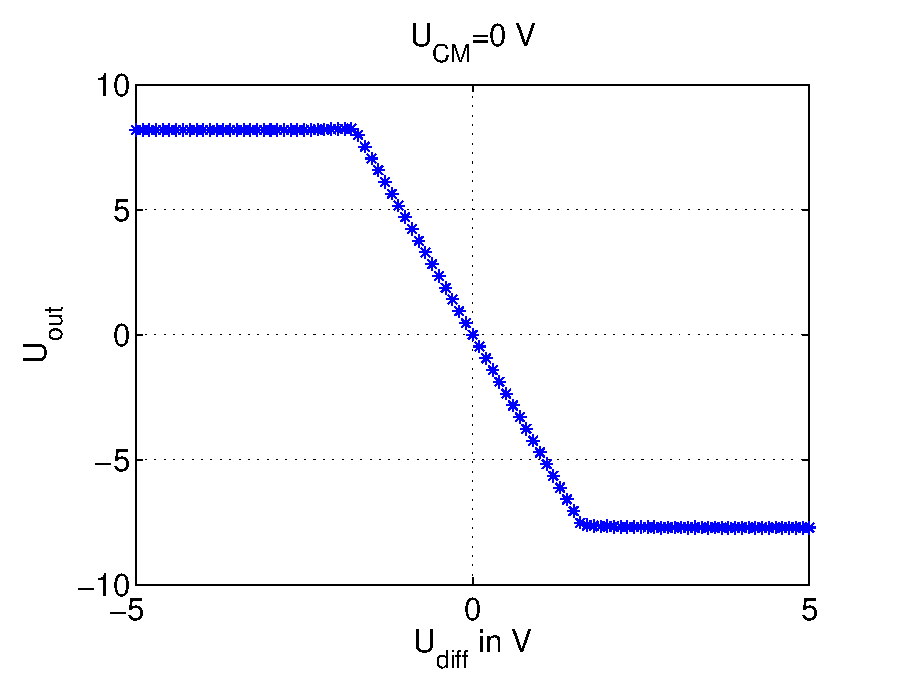
\includegraphics[scale=0.3]{./img/plots/Auf_3_Ucm_0.eps}
    \end{center}
    \end{figure}
    \begin{figure}[H]
    \begin{center}
            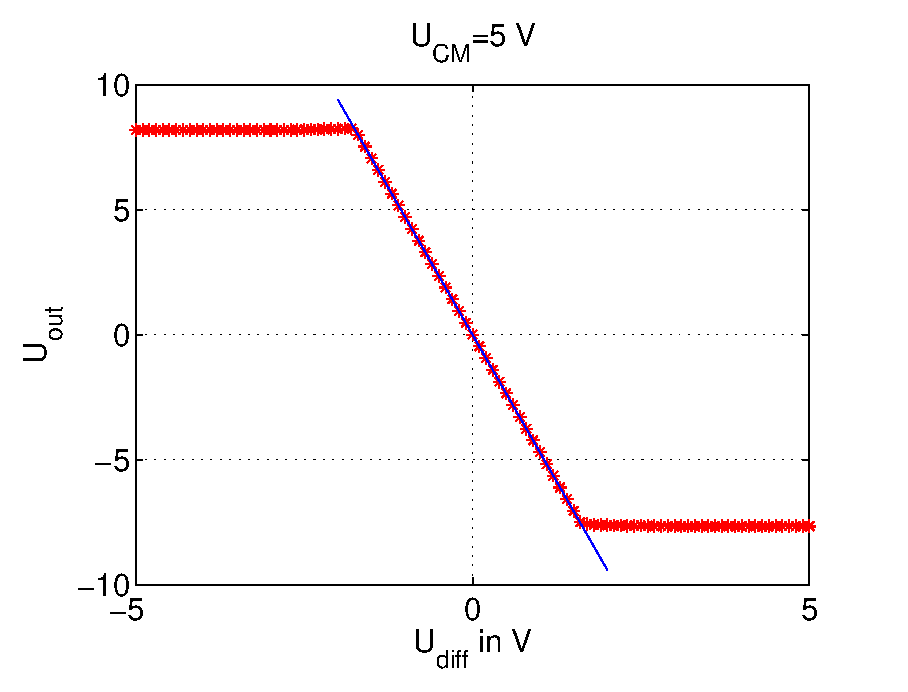
\includegraphics[scale=0.3]{./img/plots/Auf_3_Ucm_5.eps}
    \end{center}
    \end{figure}
    
    \end{columns}
\end{frame}
\begin{frame}
\frametitle{Versuchsaufbau mit Kondensator}
\framesubtitle{}
    \begin{block}{Versuch}
        \begin{itemize}
            \item Einbau von Kodensatoren und Erhöhung der Widerstände 
            \item Analyse der Schaltung
            \item Analyse des EKG-Signals
        \end{itemize}    
    \end{block}
    \begin{figure}[H]
    \begin{center}
            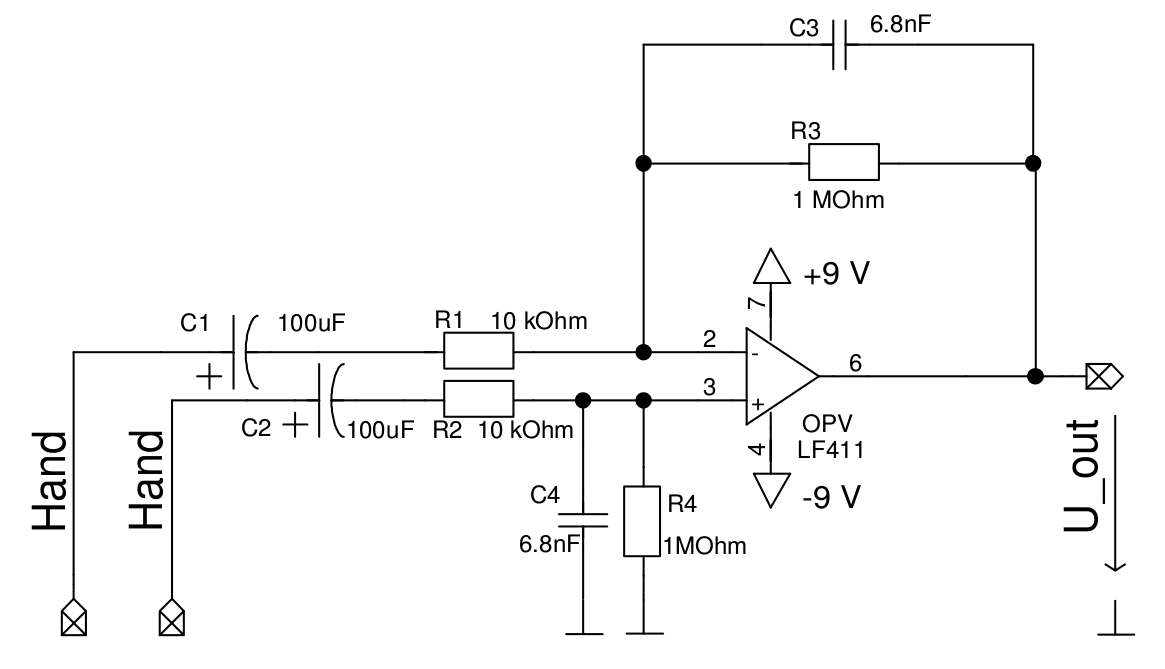
\includegraphics[scale=0.2]{./img/schaltung/dif_verst_2.png}
    \end{center}
    \end{figure}
\end{frame}
\begin{frame}
\frametitle{Übertragfunktion}
\framesubtitle{}
    \begin{block}{Übertragfunktion}
         \begin{equation*}
             | \frac{U_{in}}{U_{out}} |
             =
             \frac{1}{\sqrt{R_1^2 + \frac{1}{(2\pi f \cdot C_1}^2} \cdot
             \sqrt{\frac{1}{R_2^2}+(2\pi f \cdot C_3)^2}}
         \end{equation*}
    \end{block}
\end{frame}
\begin{frame}
\frametitle{Bodediagramm}
\framesubtitle{}
    \begin{columns}[c]
    \column{0.5\textwidth}
    \begin{block}{Ergebnis}
        \begin{itemize}
            \item Werte Stimmen nicht mit erwartetem Verlauf Überein
            \item Wahrscheinlich Fehler bei Messung (Spannung falsch
            abgegriffen)
        \end{itemize}
    \end{block}
    \column{0.5\textwidth}
    \begin{figure}[H]
    \begin{center}
            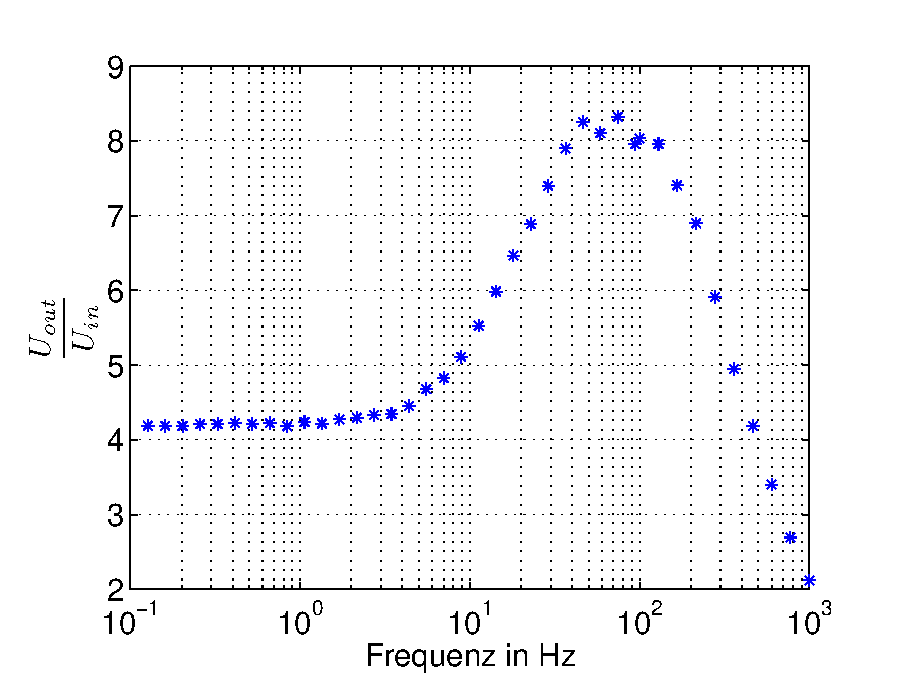
\includegraphics[scale=0.3]{./img/plots/Auf_3_bode_U.eps}
    \end{center}
    \end{figure}
    \begin{figure}[H]
    \begin{center}
            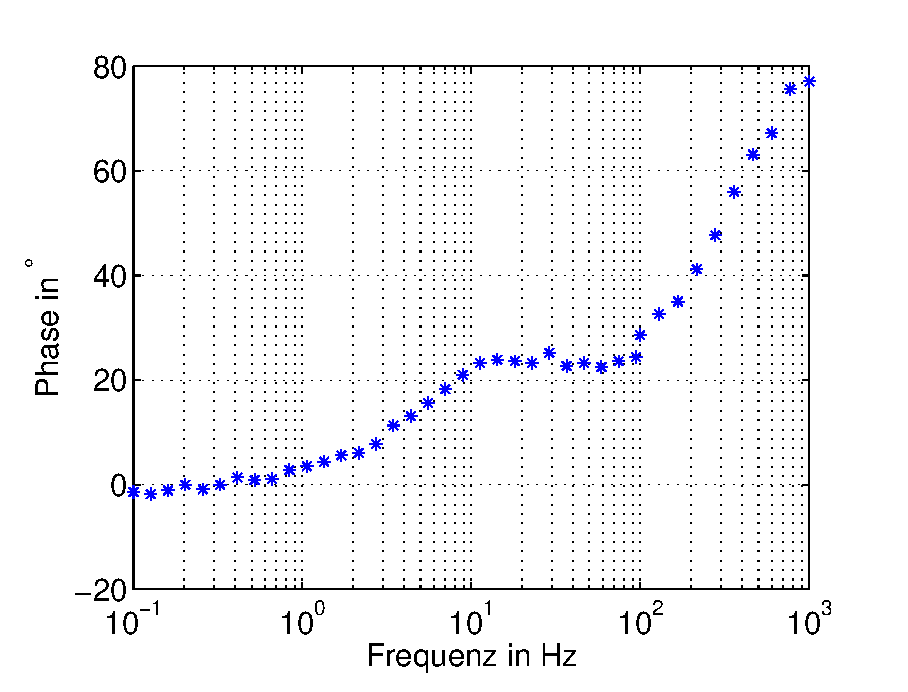
\includegraphics[scale=0.3]{./img/plots/Auf_3_bode_ph.eps}
    \end{center}
    \end{figure}
    
    \end{columns}
\end{frame}
\begin{frame}
\frametitle{Störungen im EKG}
\framesubtitle{}
\begin{figure}[H]
\begin{center}
        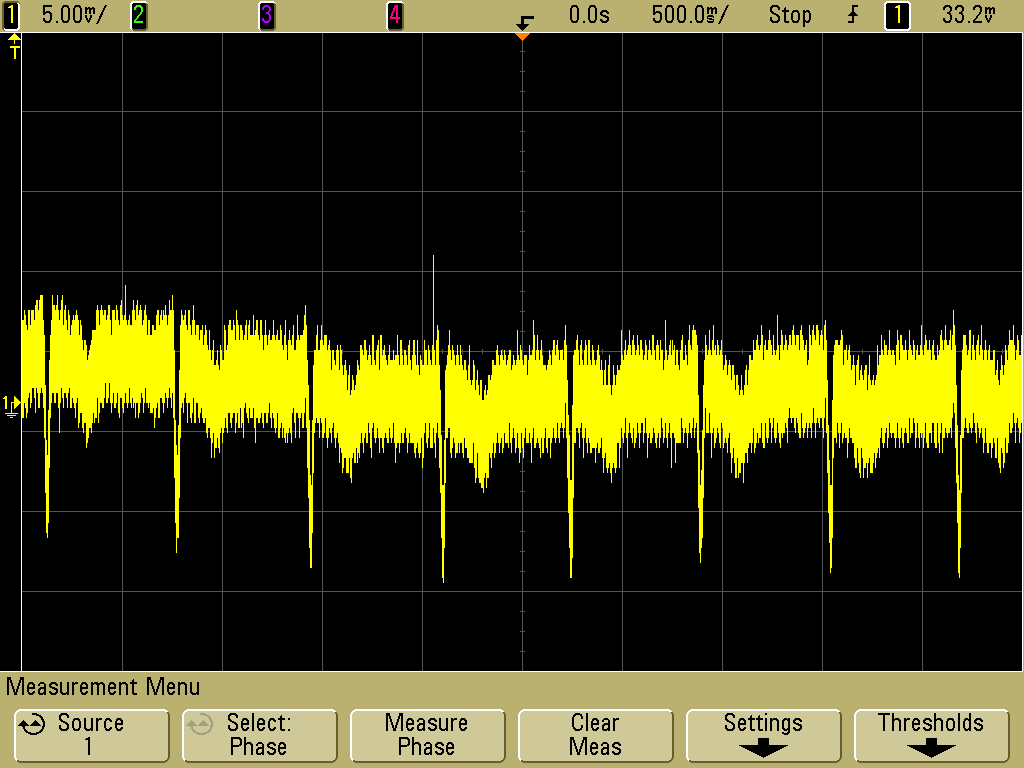
\includegraphics[scale=0.2]{./img/oszi/scope_4.png}
\end{center}
\end{figure}
\begin{block}{Herzschlag}
    \begin{itemize}
        \item Herzschlag ist erkennber 
        \item Starkes Rauschen $\rightarrow$ noch keine Messungen möglich
    \end{itemize}
\end{block}


\end{frame}
